%%%%%%%%%%%%%%%%%%%%%%%%%%%%%%%%%%%%%%%%%%%%%%%%%%%%%%%%%%%%%%%%%%%%%%%%%%%
%% This file is part of the book
%%
%% Algorithmic Graph Theory
%% http://code.google.com/p/graph-theory-algorithms-book/
%%
%% Copyright (C) 2009, 2010, 2011 Minh Van Nguyen <nguyenminh2@gmail.com>
%%
%% See the file COPYING for copying conditions.
%%%%%%%%%%%%%%%%%%%%%%%%%%%%%%%%%%%%%%%%%%%%%%%%%%%%%%%%%%%%%%%%%%%%%%%%%%%

\subfigure[December~1969]{
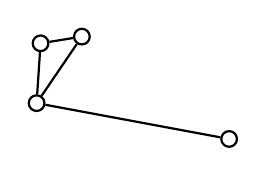
\begin{tikzpicture}
[lineDecorate/.style={-,thick},%
  nodeDecorate/.style={shape=circle,inner sep=2pt,draw,thick},
  scale=0.5]
%% nodes or vertices
\foreach \nodename/\x/\y in {
  0/2.24/6.13, 1/2.34/7.65, 2/3.39/7.82, 3/7.13/5.22}
{
  \node (\nodename) at (\x,\y) [nodeDecorate] {};
}
edges or lines
\path
\foreach \startnode/\endnode in {
  0/1, 0/2, 0/3, 1/2}
{
  (\startnode) edge[lineDecorate] node {} (\endnode)
};
\end{tikzpicture}
}
%%
%%
\qquad
\subfigure[June~1970]{
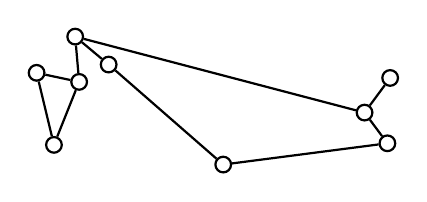
\begin{tikzpicture}
[lineDecorate/.style={-,thick},%
  nodeDecorate/.style={shape=circle,inner sep=2pt,draw,thick},
  scale=0.5]
%% nodes or vertices
\foreach \nodename/\x/\y in {
  0/1.83/7.82, 1/2.27/5.99, 2/2.91/7.59, 3/2.81/8.74, 4/3.66/8.03,
  5/6.57/5.49, 6/10.74/6.03, 7/10.16/6.81, 8/10.81/7.69}
{
  \node (\nodename) at (\x,\y) [nodeDecorate] {};
}
%% edges or lines
\path
\foreach \startnode/\endnode in {
  1/0, 1/2, 2/0, 2/3, 3/4, 4/5, 3/7, 5/6, 7/8, 7/6}
{
  (\startnode) edge[lineDecorate] node {} (\endnode)
};
\end{tikzpicture}
}
%%
%%
\qquad
\subfigure[December~1970]{
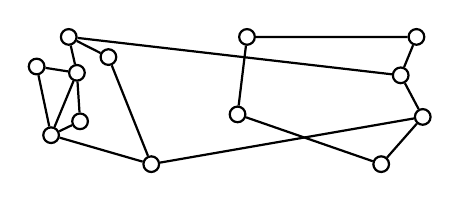
\begin{tikzpicture}
[lineDecorate/.style={-,thick},%
  nodeDecorate/.style={shape=circle,inner sep=2pt,draw,thick},
  scale=0.8]
%% nodes or vertices
\foreach \nodename/\x/\y in {
  0/2.11/5.4, 1/1.60/4.93, 2/2.24/4.83, 3/1.83/3.84, 4/2.29/4.06,
  5/2.74/5.08, 6/3.42/3.38, 7/4.79/4.17, 8/4.94/5.4, 9/7.07/3.38,
  10/7.73/4.13, 11/7.38/4.79, 12/7.63/5.4}
{
  \node (\nodename) at (\x,\y) [nodeDecorate] {};
}
%% edges or lines
\path
\foreach \startnode/\endnode in {
  3/4, 3/1, 3/2, 4/2, 1/2, 2/0, 0/5, 3/6, 5/6, 7/8, 6/10, 7/9, 9/10,
  0/11, 8/12, 11/12, 10/11}
{
  (\startnode) edge[lineDecorate] node {} (\endnode)
};
\end{tikzpicture}
}
%%
%%
\subfigure[September~1971]{
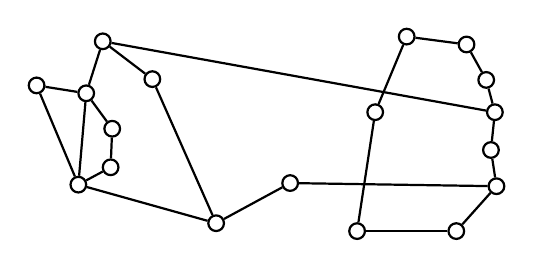
\begin{tikzpicture}
[lineDecorate/.style={-,thick},%
  nodeDecorate/.style={shape=circle,inner sep=2pt,draw,thick},
  scale=1]
%% nodes or vertices
\foreach \nodename/\x/\y in {
  0/2.01/6.27, 1/1.17/5.71, 2/1.80/5.61, 3/2.64/5.79, 4/2.13/5.16,
  5/1.70/4.45, 6/2.11/4.67, 7/3.45/3.96, 8/4.39/4.47, 9/5.47/5.37,
  10/5.24/3.86, 11/5.87/6.33, 12/6.63/6.23, 13/6.88/5.78,
  14/6.99/5.37, 15/6.94/4.89, 16/7.01/4.43, 17/6.50/3.86}
{
  \node (\nodename) at (\x,\y) [nodeDecorate] {};
}
%% edges or lines
\path
\foreach \startnode/\endnode in {
  5/6, 5/2, 5/1, 6/4, 2/1, 2/4, 2/0, 0/3, 5/7, 3/7, 7/8, 0/14, 8/16,
  10/9, 10/17, 17/16, 9/11, 11/12, 12/13, 13/14, 14/15, 15/16}
{
  (\startnode) edge[lineDecorate] node {} (\endnode)
};
\end{tikzpicture}
}
%%
%%
\qquad
\subfigure[March~1972]{
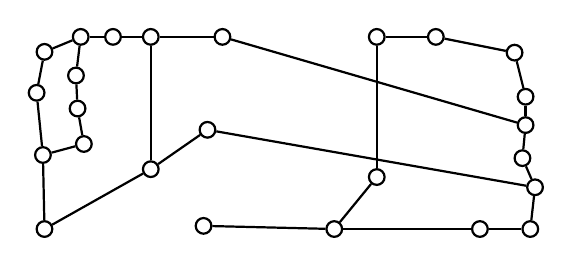
\begin{tikzpicture}
[lineDecorate/.style={-,thick},%
  nodeDecorate/.style={shape=circle,inner sep=2pt,draw,thick},
  scale=1]
%% nodes or vertices
\foreach \nodename/\x/\y in {
  0/2.03/5.21, 1/1.93/4.69, 2/2.01/3.90, 3/2.49/5.4, 4/2.9/5.4,
  5/3.38/5.4, 6/2.43/4.91, 7/2.45/4.49, 8/2.53/4.04, 9/2.03/2.96,
  10/3.38/3.72, 11/4.29/5.4, 12/4.05/3, 13/4.10/4.22,
  14/5.71/2.96, 15/6.25/3.62, 16/7.56/2.96, 17/8.20/2.96,
  18/8.26/3.49, 19/8.10/3.86, 20/8.14/4.28, 21/8.14/4.64,
  22/8/5.2, 23/7/5.4, 24/6.25/5.4}
{
  \node (\nodename) at (\x,\y) [nodeDecorate] {};
}
%% edges or lines
\path
\foreach \startnode/\endnode in {
  9/2, 9/10, 2/8, 2/1, 1/0, 7/8, 7/6, 3/0, 4/3, 4/5, 5/11, 5/10,
  10/13, 12/14, 14/15, 14/16, 13/18, 16/17, 11/20, 15/24, 24/23,
  23/22, 22/21, 21/20, 20/19, 19/18, 18/17, 3/6}
{
  (\startnode) edge[lineDecorate] node {} (\endnode)
};
\end{tikzpicture}
}
%%
%%
\subfigure[August~1972]{
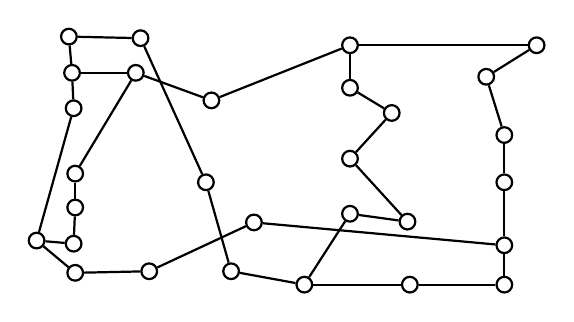
\begin{tikzpicture}
[lineDecorate/.style={-,thick},%
  nodeDecorate/.style={shape=circle,inner sep=2pt,draw,thick},
  scale=1]
%% nodes or vertices
\foreach \nodename/\x/\y in {
  0/1.20/6.85, 1/2.11/6.83, 2/1.24/6.39, 3/2.05/6.39, 4/1.26/5.94,
  5/1.28/5.11, 6/1.28/4.68, 7/0.79/4.26, 8/1.26/4.22, 9/1.28/3.85,
  10/2.22/3.87, 11/2.94/5, 12/3.01/6.04, 13/3.26/3.87,
  14/3.55/4.49, 15/4.19/3.70, 16/4.77/4.6, 17/5.53/3.70,
  18/5.5/4.5, 19/4.77/5.3, 20/5.30/5.88, 21/4.77/6.2,
  22/4.77/6.74, 23/7.14/6.74, 24/6.5/6.34, 25/6.73/5.6,
  26/6.73/5, 27/6.73/4.2, 28/6.73/3.70}
{
  \node (\nodename) at (\x,\y) [nodeDecorate] {};
}
%% edges or lines
\path
\foreach \startnode/\endnode in {
  9/7, 7/8, 7/4, 8/6, 6/5, 5/3, 4/2, 2/3, 2/0, 1/0, 1/11, 10/9, 10/14,
  3/12, 12/22, 11/13, 13/15, 15/17, 17/28, 14/27, 15/16, 16/18, 18/19,
  19/20, 20/21, 21/22, 28/27, 27/26, 26/25, 25/24, 24/23, 23/22}
{
  (\startnode) edge[lineDecorate] node {} (\endnode)
};
\end{tikzpicture}
}
%%
%%
\qquad
\subfigure[September~1973]{
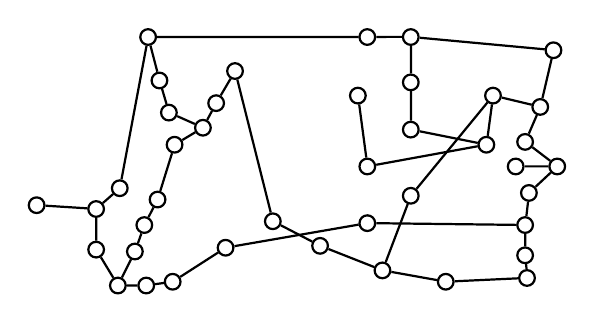
\begin{tikzpicture}
[lineDecorate/.style={-,thick},%
  nodeDecorate/.style={shape=circle,inner sep=2pt,draw,thick},
  scale=1.2]
%% nodes or vertices
\foreach \nodename/\x/\y in {
  0/4.18/5.68, 1/4.30/5.22, 2/4.40/4.88, 3/4.90/4.98, 4/5.10/5.32,
  5/4.76/4.72, 6/4.46/4.54, 7/3.88/4.08, 8/3.63/3.86, 9/3/3.90,
  10/4.28/3.96, 11/4.14/3.69, 12/3.63/3.43, 13/4.04/3.41,
  14/3.86/3.05, 15/4.16/3.05, 16/4.44/3.09, 17/5/3.45,
  18/5.5/3.73, 19/6/3.47, 20/6.5/3.71, 21/6.66/3.21,
  22/6.96/4, 23/7.33/3.09, 24/8.19/3.13, 25/8.17/3.37,
  26/8.17/3.69, 27/8.21/4.03, 28/8.51/4.31, 29/8.07/4.31,
  30/8.17/4.57, 31/8.33/4.94, 32/7.83/5.06, 33/7.76/4.54,
  34/6.96/4.7, 35/6.96/5.2, 36/6.96/5.68, 37/6.5/5.68,
  38/8.47/5.54, 39/6.5/4.31, 40/6.4/5.06}
{
  \node (\nodename) at (\x,\y) [nodeDecorate] {};
}
%% edges or lines
\path
\foreach \startnode/\endnode in {
  14/15, 15/16, 14/13, 14/12, 12/8, 8/9, 8/7, 13/11, 11/10, 10/6, 6/5,
  7/0, 5/2, 2/1, 1/0, 5/3, 3/4, 0/37, 4/18, 16/17, 17/20, 18/19,
  19/21, 21/23, 21/22, 23/24, 24/25, 25/26, 20/26, 26/27, 27/28,
  28/29, 28/30, 22/32, 30/31, 31/32, 31/38, 32/33, 33/34, 34/35,
  35/36, 36/37, 36/38, 33/39, 39/40}
{
  (\startnode) edge[lineDecorate] node {} (\endnode)
};
\end{tikzpicture}
}
%%
%%
\subfigure[June~1974]{
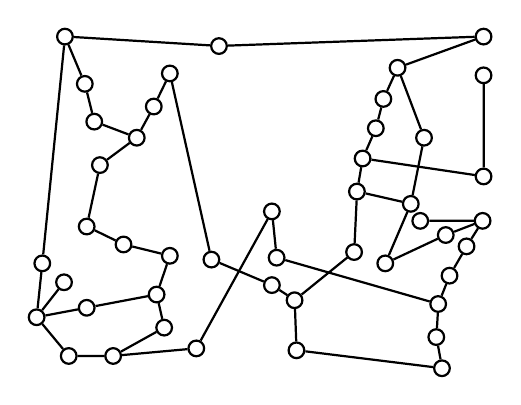
\begin{tikzpicture}
[lineDecorate/.style={-,thick},%
  nodeDecorate/.style={shape=circle,inner sep=2pt,draw,thick},
  scale=1.2]
%% nodes or vertices
\foreach \nodename/\x/\y in {
  0/2.2/4, 1/1.91/3.63, 2/1.97/4.20, 3/2.21/6.60, 4/2.42/6.10,
  5/2.52/5.70, 6/3.32/6.21, 7/3.15/5.86, 8/2.97/5.53, 9/2.58/5.24,
  10/2.44/4.59, 11/2.83/4.40, 12/3.32/4.28, 13/3.18/3.87,
  14/2.44/3.73, 15/2.25/3.22, 16/2.72/3.22, 17/3.26/3.52,
  18/3.6/3.3, 19/3.76/4.24, 20/3.84/6.5, 21/4.4/3.97,
  22/4.4/4.75, 23/4.45/4.26, 24/4.64/3.81, 25/5.27/4.32,
  26/4.66/3.28, 27/6.20/3.09, 28/6.14/3.42, 29/6.16/3.77,
  30/6.28/4.07, 31/6.46/4.38, 32/5.97/4.65, 33/6.63/4.65,
  34/6.24/4.5, 35/5.6/4.2, 36/5.87/4.83, 37/5.30/4.96,
  38/5.36/5.31, 39/5.50/5.63, 40/6.64/5.12, 41/6.01/5.53,
  42/5.58/5.94, 43/5.73/6.27, 44/6.64/6.19, 45/6.64/6.6}
{
  \node (\nodename) at (\x,\y) [nodeDecorate] {};
}
%% edges or lines
\path
\foreach \startnode/\endnode in {
  1/0, 1/2, 1/15, 1/14, 16/15, 16/17, 16/18, 13/14, 13/17, 13/12, 3/4,
  3/2, 3/20, 11/10, 11/12, 9/10, 9/8, 5/4, 5/8, 7/8, 7/6, 19/6, 19/21,
  45/20, 45/43, 22/18, 22/23, 24/21, 24/25, 24/26, 27/26, 27/28,
  29/23, 29/28, 29/30, 31/30, 31/33, 33/32, 33/34, 35/34, 35/36,
  37/25, 37/36, 37/38, 41/36, 41/43, 43/42, 42/39, 39/38, 40/38, 40/44}
{
  (\startnode) edge[lineDecorate] node {} (\endnode)
};
\end{tikzpicture}
}
%%
%%
\qquad
\subfigure[July~1975]{
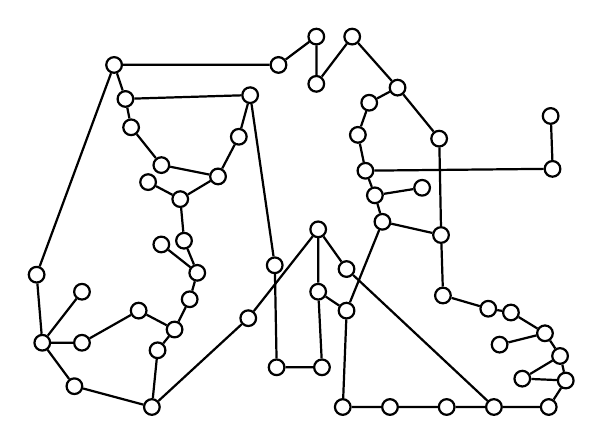
\begin{tikzpicture}
[lineDecorate/.style={-,thick},%
  nodeDecorate/.style={shape=circle,inner sep=2pt,draw,thick},
  scale=1.2]
%% nodes or vertices
\foreach \nodename/\x/\y in {
  0/2.14/3.8, 1/1.72/3.26, 2/2.06/2.80, 3/2.88/2.58, 4/2.94/3.18,
  5/3.12/3.40, 6/2.74/3.60, 7/2.14/3.26, 8/1.66/3.98, 9/3.28/3.72,
  10/3.36/4.00, 11/2.98/4.30, 12/3.22/4.34, 13/2.84/4.96,
  14/3.18/4.78, 15/3.58/5.02, 16/2.98/5.14, 17/2.66/5.54,
  18/2.60/5.84, 19/2.48/6.2, 20/3.80/5.44, 21/3.92/5.88,
  22/3.9/3.52, 23/4.18/4.08, 24/4.22/6.2, 25/4.2/3.0,
  26/4.68/3.0, 27/4.64/4.46, 28/4.64/3.80, 29/4.94/4.04,
  30/4.62/6.5, 31/4.62/6.0, 32/5/6.5, 33/5.48/5.96,
  34/5.18/5.80, 35/5.06/5.46, 36/5.14/5.08, 37/5.92/5.42,
  38/5.74/4.90, 39/5.24/4.82, 40/5.32/4.54, 41/5.94/4.40,
  42/4.94/3.6, 43/4.9/2.58, 44/5.96/3.76, 45/5.4/2.58,
  46/6/2.58, 47/6.5/2.58, 48/7.08/2.58, 49/6.80/2.88,
  50/7.26/2.86, 51/7.20/3.12, 52/6.56/3.24, 53/7.04/3.36,
  54/6.68/3.58, 55/6.44/3.62, 56/7.12/5.10, 57/7.10/5.66}
{
  \node (\nodename) at (\x,\y) [nodeDecorate] {};
}
%% edges or lines
\path
\foreach \startnode/\endnode in {
  1/0, 1/8, 1/2, 1/7, 19/8, 19/24, 19/18, 6/5, 6/7, 3/2, 3/4, 3/22,
  5/4, 5/9, 9/10, 17/18, 17/16, 10/11, 10/12, 14/13, 14/12, 14/15,
  15/16, 15/20, 21/18, 21/20, 21/23, 25/23, 25/26, 27/22, 27/28,
  27/29, 28/26, 28/42, 30/24, 30/31, 32/31, 32/33, 33/34, 34/35,
  35/36, 36/39, 40/39, 40/42, 40/41, 43/42, 43/45, 29/47, 38/39,
  37/33, 37/41, 56/36, 56/57, 44/41, 44/55, 46/45, 46/47, 54/55,
  54/53, 53/52, 53/51, 51/49, 51/50, 50/49, 50/48, 48/47}
{
  (\startnode) edge[lineDecorate] node {} (\endnode)
};
\end{tikzpicture}
}
%%
%%
\subfigure[July~1976]{
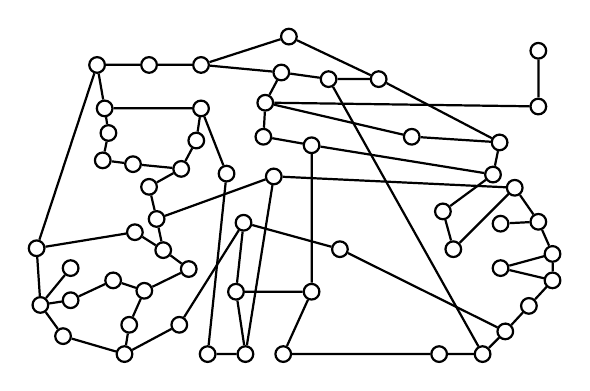
\begin{tikzpicture}
[lineDecorate/.style={-,thick},%
  nodeDecorate/.style={shape=circle,inner sep=2pt,draw,thick},
  scale=1.2]
%% nodes or vertices
\foreach \nodename/\x/\y in {
  0/1.65/3.9, 1/1.33/3.51, 2/1.29/4.11, 3/1.57/3.18, 4/1.65/3.56,
  5/2.22/2.99, 6/2.27/3.3, 7/2.10/3.77, 8/2.43/3.66, 9/2.9/3.89,
  10/2.63/4.09, 11/2.33/4.28, 12/2.56/4.42, 13/2.48/4.76,
  14/1.99/5.04, 15/2.31/5.0, 16/2.05/5.33, 17/2.01/5.59, 18/1.93/6.05,
  19/2.82/4.95, 20/2.98/5.25, 21/3.03/5.59, 22/2.8/3.3,
  23/3.3/4.9, 24/2.48/6.05, 25/3.1/2.99, 26/3.8/4.87,
  27/3.5/2.99, 28/3.48/4.38, 29/3.4/3.65, 30/4.5/4.1,
  31/3.03/6.05, 32/3.96/6.35, 33/4.91/5.9, 34/4.38/5.9,
  35/3.88/5.97, 36/3.71/5.65, 37/3.69/5.29, 38/4.2/5.2,
  39/4.2/3.65, 40/3.9/2.99, 41/5.55/2.99, 42/6.01/2.99,
  43/6.25/3.23, 44/6.5/3.5, 45/6.75/3.77, 46/6.2/3.9,
  47/6.75/4.05, 48/6.2/4.37, 49/6.6/4.39, 50/6.35/4.75,
  51/5.7/4.1, 52/5.59/4.5, 53/6.12/4.89, 54/5.26/5.29,
  55/6.19/5.23, 56/6.6/5.61, 57/6.6/6.2}
{
  \node (\nodename) at (\x,\y) [nodeDecorate] {};
}
%% edges or lines
\path
\foreach \startnode/\endnode in {
  1/0, 1/2, 1/4, 1/3, 5/3, 5/6, 7/4, 7/8, 8/6, 8/9, 11/2, 11/10, 10/9,
  10/12, 18/2, 18/17, 18/24, 14/16, 14/15, 17/16, 17/21, 13/12, 13/19,
  19/15, 19/20, 21/20, 21/23, 22/5, 22/28, 26/12, 25/23, 25/27, 26/27,
  26/50, 29/27, 29/28, 29/39, 30/28, 30/43, 31/24, 31/35, 32/31,
  32/33, 34/33, 34/35, 34/42, 35/36, 36/37, 37/38, 39/38, 39/40,
  41/40, 41/42, 42/43, 43/44, 44/45, 46/45, 46/47, 47/45, 47/49,
  49/48, 49/50, 51/52, 51/50, 53/38, 53/52, 53/55, 54/36, 54/55,
  55/33, 56/36, 56/57}
{
  (\startnode) edge[lineDecorate] node {} (\endnode)
};
\end{tikzpicture}
}
